\chapter{Theoretical background}
In this chapter, we will give an overview of the theoretical background necessary for Higgs boson searches at the LHC. We will start with an overview of the standard model (SM) of particle physics, followed by a description of the phenomenology for proton-proton collisions and Higgs boson production. We conclude with a discussion on the relevance of the search for the associated production of the Higgs boson with top quarks.

\section{Standard Model}
The fundamental building blocks of the SM are quantum fields~$\phi(x)$~that depend on space-time coordinates~$x$. The interaction of these fields is governed by Quantum Field Theory (QFT), which is a Lorentz-invariant theory of quantum-mechanics. These fields can be classified according to their transformation properties under various symmetry groups, in particular, the Lorentz group and thus associated to particles. The principle of gauge invariance allows us to use these transformation properties to describe fundamental interactions via particle exchange. Much of particle physics is concerned with the measurement of decay rates and scattering cross sections, which are computed using perturbation series in QFT.

The particle content of the SM is summarized on~\cref{fig:standard_model}.

\begin{figure}
\begin{centering}
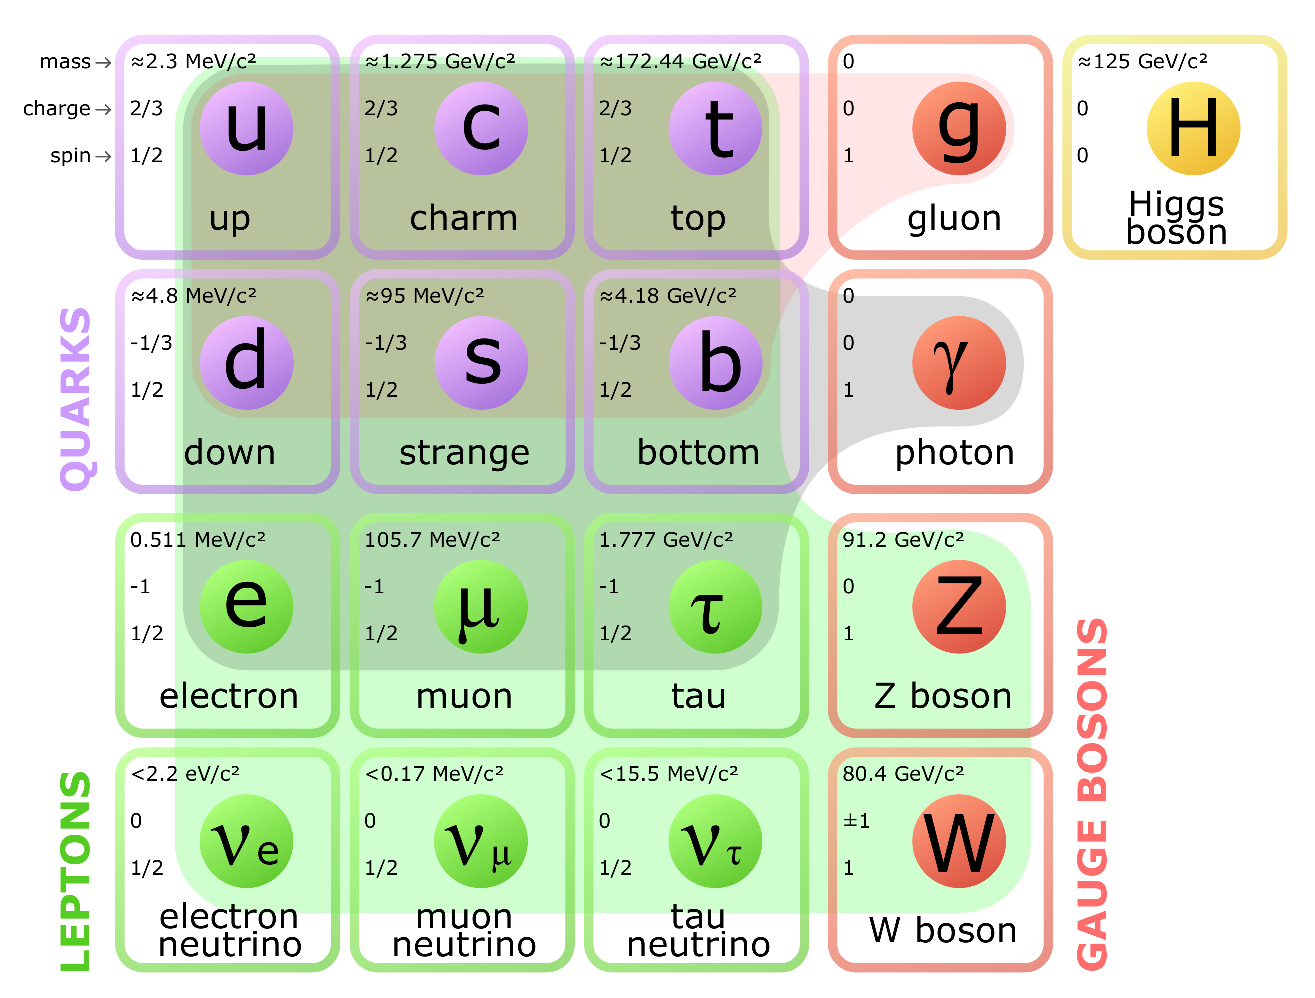
\includegraphics[width=0.6\textwidth]{figures/theory/Standard_Model_of_Elementary_Particles_modified_version.eps}
\caption[The particle content of the Standard Model]{The particle content of the Standard Model. Figure adapted from~\cite{wikipediaSM}.}
\label{fig:standard_model}
\end{centering}
\end{figure}


\section{The Lorentz group and particle states}

Lorentz group consists of coordinate transformations~$x^\mu = \Lambda^{\mu}_{\ \nu} x^\nu$~that preserve space-time intervals~$\mathrm{d}s^2 = \mathrm{d}x^\mu \Lambda^\mu_{\ \nu} x_\nu$, such that~$\mathrm{det}\ \Lambda = +1$~and~$\mathrm{sign}\ \Lambda^0_{\ 0} = +1$. The transformations form a group~$\mathrm{SO}^+(3,1)$, which can be decomposed~$\mathrm{SO}^+(3,1) \simeq \mathrm{SU}(2)_L \times \mathrm{SU}(2)_R$. The angular momenta~$(j_1, j_2)$~can be used to group the fields as scalars, left and right handed spinors and vectors. For example, a scalar field~$\phi(x)$~transforms as~$\phi(x) \rightarrow \phi(\Lambda^{-1} x)$, a vector field as~$A^\mu(x) \rightarrow \Lambda^\mu_{\ \nu} A^\nu(\Lambda^{-1}x)$~and a spinor field as~$\phi^\alpha(x) = S[\Lambda]^a_{\ \beta} \phi^\beta(x)$, where~$S[\Lambda]$~is a spinor representation built from~$4\times4$~Dirac~$\gamma$~matrices in the chiral representation.

These fields can be identified with particle states, which have a definite mass~$m$~and spin~$s$. Particles with integer spin follow Bose-Einstein statistics and are therefore called bosons, whereas particles with half-integer follow Fermi-Dirac statistics and are called fermions. 

\section{Relativistic quantum mechanics}
After having identified quantum fields with definite Lorentz transformation properties as central to QFT, the next step is to derive dynamical relations for the free fields in order to describe the propagation of free particles.

The Klein-Gordon wave equation,

\begin{equation}
\label{eq:theory_klein_gordon}
(\partial^\mu \partial_\mu + m^2) \psi = 0
\end{equation}
which can be derived from Einstein's energy-momentum relation~$E^2 = \vec{p}^2 + m^2$~by replacing energy and momentum with operators acting on the wavefunction~$\psi$, is a manifestly Lorentz-invariant relation between energy and momentum for the quantum mechanical wavefunction. However, it admits solutions with negative energy and negative probability densities, which are unphysical.

These negative-probability states led Dirac to search for a relation linear in~$\hat{\mathbf{p}}$~and~$E$, which resulted in the Dirac equation:

\begin{equation}
\label{eq:theory_dirac}
i (\gamma^\mu \partial_\mu - m) \psi = 0
\end{equation}
where~$\gamma^\mu$~are the~$4\times4$~Dirac~$\gamma$-matrices which satisfy the Clifford algebra anti-commutation relation~$\{ \gamma^\mu, \gamma^\nu \} = \gamma^\mu \gamma^\nu + \gamma^\nu \gamma^\mu = 2 g^{\mu\nu} \mathbb{I}$~and~$\psi$~is a four-component spinor. Using~\cref{eq:theory_dirac}, we can describe the dynamics, spin and magnetic momentum of free spin-half fermions. The probability densities predicted by Dirac's equation are now positive, but it still admits solutions with negative energy. In the Feynman-Stückelberg interpretation, these~$E<0$~particles can be interpreted as negative-energy particles moving backwards in time or equivalently anti-particles moving forwards in time. The predictions by Dirac's equation were spectacularly confirmed by the discovery of the positron in 1932~\cite{anderson1933positive}.

Both of these equations of motion can be derived using the principle of least action:

\begin{equation}
\label{eq:theory_action}
S = \int \mathrm{d}^4x\ \mathcal{L}_{\mathrm{free}},\ \delta S = 0,
\end{equation}
where~$\mathcal{L}_{\mathrm{free}}$~is the Lagrangian density for non-interacting fields. The Dirac action for a single free spinor field can be written as

\begin{equation}
\label{eq:theory_kg_lagrangian}
\mathcal{L}_{\mathrm{Dirac}} = \bar{\psi} i \gamma^\mu \partial_\mu \psi - m \bar{\psi} \psi,\ \bar{\psi} = \psi^\dagger \gamma^0
\end{equation}
and varied with respect to~$\psi$~to derive the Dirac equation.

\section{Interactions via gauge theory}
The concept of interactions mediated by fields is central to QFT and they can be described by requiring the Lagrangian to have additional symmetries. In particular, if we require the laws of physics to be invariant under local transformations~$\psi(x) \rightarrow U(x) \psi(x)$, where the continuous and differentiable transformations~$U(x)$~form Lie groups, then additional degrees of freedom corresponding to the mediator fields or gauge bosons are naturally incorporated in the Lagrangian.

\subsection{Quantum Electrodynamics}
For the~$\mathrm{U}(1)$~symmetry, which corresponds to the transformation~$\psi(x) \rightarrow e^{i q\varphi(x)} \psi(x)$, the derivative in the momentum operator in~\cref{eq:theory_kg_lagrangian} needs to be changed to

\begin{equation}
\partial_{\mu} \rightarrow \partial_{\mu} + i q A_{\mu}
\end{equation}
in order for the Lagrangian to be invariant under this symmetry. The field~$A_{\mu}$~is a massless gauge boson with spin 1 that is coupled to the fermion field~$\psi$~via a coupling constant~$q$~in the term~$q \gamma^\mu A_\mu \psi$. The formulation of quantum electrodynamics (QED) as a gauge theory generated by the Abelian group~$\mathrm{U}(1)_{\mathrm{EM}}$~was first done by Tomonaga, Feynman and Schwinger. In QED, the spinor~$\psi$~is associated to the electron, the vector~$A_\mu$~to the photon and~$q$~is the electric charge of the fermion. 

In order to compute observable decay rates or scattering cross sections under an interacting Hamiltonian~$H$, we use Fermi's golden rule, which relates the scattering rate~$\Gamma_{fi}$~to the transition matrix element between the initial and final state derived using perturbation theory:

\begin{equation}
\label{eq:transition_matrix}
\mathcal{M}_{fi} = \langle \psi_f | H | \psi_i \rangle.
\end{equation}

The matrix element~\cref{eq:transition_matrix} is a Lorentz scalar and can be explicitly computed from the Lagrangian using Feynman rules, where we represent each term in the perturbation expansion of~\cref{eq:transition_matrix} as a graphical diagram with the ingoing and outgoing lines, the vertices and the propagators are associated with quantities that are specified by the Lagrangian. The QED interaction vertex thus allows us to construct diagrams corresponding to any QED interaction and calculate scattering cross sections for processes such as electron-electron scattering, as depicted on~\cref{fig:theory_qed}.

\begin{figure}
\begin{centering}
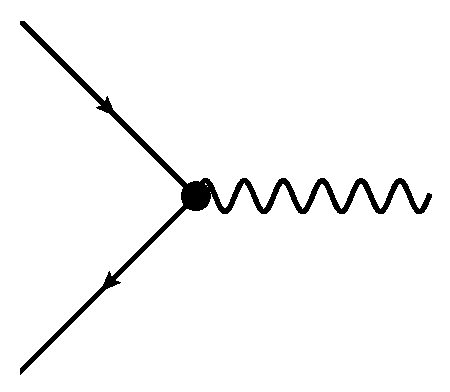
\includegraphics[width=0.3\textwidth]{figures/theory/qed_vertex.eps}
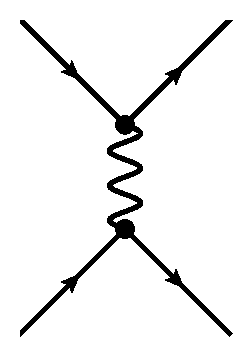
\includegraphics[width=0.2\textwidth]{figures/theory/qed_process.eps}
\caption{The QED vertex and a representative process.}
\label{fig:theory_qed}
\end{centering}
\end{figure}

It is remarkable that the gauge theory formulation of QED allows us to both recover Maxwell's equations of electromagnetism and predict the anomalous electric dipole moment of the electron, which has been confirmed to be accurate to about one part per billion. This underscores the predictive power of symmetries in the SM.

\subsection{Quantum chromodynamics}
\label{sec:theory_qcd}
The interaction of quarks and gluons can be described by the theory of quantum chromodynamics (QCD), which arises from the invariance of the Lagrangian under a local~$\mathrm{SU}(3)_C$~symmetry, where C stands for a colour charge that is~$N_c$-valent, with~$N_c = 3$~in the SM. The spinor field transforms under this group as

\begin{equation}
\psi(x) \rightarrow \psi'(x) = \exp \bigl[ i g_s \alpha^a(x) T^a \bigr] \psi(x)
\end{equation}
where~$T_a$~are the generators of the group represented by the~$3\times3$~Gell-Mann matrices~$\lambda^a$~as~$T_a = \frac{1}{2} \lambda^a$,~$g_s$~is the gauge coupling and~$\alpha^a(x)$~are the local gauge transformations corresponding to the 8 generators. The derivative can then be written as


\begin{equation}
\label{eq:theory_qcd_deriv}
\partial_\mu \rightarrow \partial_\mu + i g_s G^a_\mu T^a
\end{equation}
where~$G^a_\mu = \partial_\mu \alpha^a(x)$~must transform as~$G^a_\mu \rightarrow G^a_\mu - \partial_\mu \alpha^a - g_s f_{ijk} \alpha^i G^j_\mu$. The last term arises due to the non-Abelian nature of QCD, which means that the generators~$T^a$~do not commute, but are instead related through the structure constants:~$[T^a, T^b] = 2 i f_{abc} T^c$. The Lagrangian for a single quark field can then be written as

\begin{equation}
\label{eq:theory_quark_lagrangian}
\mathcal{L}_{\mathrm{quark}} = \bar{\Psi} (i \gamma^\mu \partial_\mu - m + g_s \gamma^\mu G^a_\mu T^a) \Psi = 0
\end{equation}
and we can associate~$G^a_\mu$~to the gluons and note that~$\Psi = (\psi_i)$~have 3 components corresponding to colour states, each of which is a 4-component Dirac spinor. The QCD quark-gluon interaction vertex is then

\begin{equation}
g_s \gamma_\mu T^a G^a_\mu.
\end{equation}

At this stage,~$G^a_\mu$~is simply a field associated with external sources, which can be made dynamical by adding a gauge-invariant term

\begin{equation}
\mathcal{L}_{\mathrm{gauge}} = - \frac{1}{2} \mathrm{Tr}\ [F^{\mu\nu} F_{\mu\nu}] 
\end{equation}
to the QCD Lagrangian, where~$F_{\mu\nu} = \partial_\mu G_\nu - \partial_\nu G_\mu + i g_s [G_\mu, G_\nu]$~with~$G_\mu = G_\mu^a T^a$~is the QCD gluon field strength tensor.

The~$\mathrm{SU}(3)_{\mathrm{C}}$~symmetry of QCD thus implies the existence of a conserved colour charge, which is exchanged between quarks by 8 gluons in QCD vertices. As free quarks have not been experimentally detected, the colour charge is hypothesised to be confined, such that quarks are only observed bound to colourless hadrons. Furthermore, this means that hadrons have to be colour singlets, which for baryons, composed of 3 quarks, implies that the colour wavefunction must be totally antisymmetric under the exchange of any two quarks, since the colour  singlet~$\psi_c = \frac{1}{\sqrt{6}} (rgb - rbg + gbr - grb + brg - bgr)$~from the decomposition~$\mathbf{3}\otimes \mathbf{3} \otimes \mathbf{3} = \mathbf{10} \oplus \mathbf{8} \oplus \mathbf{8} \oplus \mathbf{1}$~is totally antisymmetric.

In order to describe the phenomenology of high-energy interactions of protons, we thus need an effective model for building hadrons out of the elementary constituents of QCD - the quarks and gluons.

\section{The parton model}
Through the study of deep inelastic scattering (DIS) experiments, where an electron transfers sufficient energy~$Q^2$~to a proton for it to break up in the reaction~$\mathrm{e}^- \mathrm{p} \rightarrow \mathrm{e}^- \mathrm{X}$, it was possible to establish that the electrons scatter elastically off point-like spin-half constituents of the proton, the partons. This can be seen as an analogy to the Rutherford experiment, where electrons were scattered off the nucleus of an atom to reveal the pointlike structure of the nucleus within. By identifying the partons as the quarks from QCD, electron-proton interactions can thus be described in terms of the more fundamental electron-quark interactions.

Furthermore, by measuring the~$Q^2$-dependence of the QCD coupling constant~$\alpha_s(Q^2) = q^2 / 4\pi$~ experimentally and from theoretical considerations of QCD~\cite{PhysRevLett.30.1343,PhysRevLett.30.1346}, it has been possible to establish that at very high~$Q^2$, the coupling constant~$\alpha_S(Q^2)$~becomes vanishingly small, such that quarks can be treated as free particles in the asymptotic limit. The~$Q^2$-dependence of~$\alpha_s$~can be seen on~\cref{fig:theory_alphas_running}, confirming the QCD prediction of asymptotic freedom. Only when the coupling~$\alpha_S(Q^2)$~is sufficiently small can perturbative QCD (pQCD) be used to compute cross-sections of the underlying processes. At a momentum scale comparable to typical hadron sizes~$\Lambda_{\mathrm{QCD}} = 0.1\dots0.3$~GeV, the coupling constant becomes unphysical, implying the breakdown of perturbative QCD at~$Q < \Lambda_{\mathrm{QCD}}$.

\begin{figure}
\begin{centering}
\includegraphics[width=1.0\textwidth]{figures/theory/asq-2015.pdf}
\caption[The measured values of~$\alpha_S(Q^2)$ compared to NLO QCD]{The measured values of~$\alpha_S(Q^2)$, compared to the prediction from NLO QCD. Figure from~\cite{Patrignani:2016xqp}.}
\label{fig:theory_alphas_running}
\end{centering}
\end{figure}

In order to model a proton-proton interaction with a hard scattering, such as the Drell-Yan process~$\mathrm{q} \bar{\mathrm{q}} \rightarrow \ell^+ \ell^-$~at high~$Q^2$, we describe the protons in terms of parton distribution functions~(PDFs)~$f_a^{\mathrm{p}}(x)$, which specify the fraction of proton momentum~$x$~carried by a quasi-free constituent quark or gluon~$a$~and factorize the proton-proton interaction to a hard interaction between quarks and gluons, as depicted on~\cref{fig:theory_pdf_factorization}. This allows us to write the factorized cross-section as


\begin{equation}
\label{eq:theory_pdf_factorization}
\mathrm{d}\sigma(\mathrm{p}\mathrm{p} \rightarrow cd) = \int_0^1 \mathrm{d}x_1 \mathrm{d}x_2 \sum_{a,b} f_a^{\mathrm{p}}(x_1, \mu_F^2) f_b^{\mathrm{p}}(x_2, \mu_F^2)\ \mathrm{d}\hat{\sigma}^{ab \rightarrow cd} (Q^2, \mu_f^2),
\end{equation}
which is evaluated at the factorization scale~$\mu_f^2$. The PDFs have to be determined from experimental data. As the proton is a dynamical system of bound quarks that interact strongly via virtual gluon exchange, the protons are found to contain a \textit{sea} of gluons and quarks and anti-quarks from the vacuum fluctuations of~$g \rightarrow \mathrm{q} \bar{\mathrm{q}}$~in addition to the up and down \textit{valence} quarks expected from flavour symmetry.

\section{Flavour states of hadrons}
The known quarks of the SM come in 6 different flavours, grouped into 3 generations: up and down (I), charm and strange (II), top and bottom (III). The underlying reason for the SM having exactly 3 generations is unknown, but an approximate symmetry between flavours allows us to predict allowable hadronic states that can be formed from quarks. Strong interaction is approximately invariant under~$\mathrm{u} \leftrightarrow \mathrm{d}$~exchange, which implies an~$\mathrm{SU}(2)$~flavour symmetry. This group has 3 generators~$\hat{T}_i$~that can be represented as~$2\times2$~Pauli spin matrices. This means that for a given flavour state~$\psi$, the quantized isospin~$I_3 \leftrightarrow \hat{T}_3$~and the total isospin~$I \leftrightarrow \hat{T}^2$~are conserved in analogy to spin, and can therefore be used to label composite flavour states of quarks as~$\phi(I, I_3)$.

We can construct the flavour wavefunction proton, which contains 3 valence quarks (uud), by combining 3 isospin doublets~$\mathbf{2} \otimes \mathbf{2} \otimes \mathbf{2}$, which results in a spin~$I=3/2$~quadruplet and two spin~$I=1/2$~doublets~$\phi_A=\frac{1}{\sqrt{2}}(\mathrm{udu} - \mathrm{duu})$~and~$\phi_S = \frac{1}{\sqrt{6}}(2 \mathrm{uud} - \mathrm{duu} - \mathrm{udu})$, that are (anti)symmetric under the exchange of the first two quarks. The proton wavefunction is then a superposition of the two flavour doublets, multiplied by the corresponding (anti)symmetric wavefunctions for the spin states, such that the flavour-spin wavefunction is completely symmetric under the exchange of any two quarks. This, combined with the completely antisymmetric colour wavefunction as described in~\cref{sec:theory_qcd}, guarantees that the proton wavefunction is completely antisymmetric under the exchange of any two quarks.

The~$\mathrm{SU}(2)$~isospin symmetry of flavour allows us to write down the wavefunction of the proton in the ground state and predict the existence and approximate masses of the excited states such as the~$\Delta$-baryons. It is not an exact symmetry, as illustrated by the difference in the proton and neutron masses, which should vanish under precise~$\mathrm{SU}(2)$~isospin symmetry, but nevertheless underscores the role of symmetries in describing hadronic states.

\section{Electroweak unification}
The parity-violating weak force, which couples neutrinos to charged leptons and is responsible for radioactive~$\beta$-decay, can be associated to a~$\mathrm{SU}(2)_L$~gauge symmetry. The left-handed fermions form doublets~$(\nu_L, \mathrm{\ell}_L)$~for leptons and~$(q_L, q'_L)$~for quarks, whereas right-handed fermions are singlets under weak isospin. The generators~$T^i$~of~$\mathrm{SU}(2)_L$~are related to the 3 Pauli matrices~$T_i = \frac{1}{2}\sigma_i$, which can then be associated to 3 vector boson fields that mediate the weak force:~$W^+_\mu, W^-_\mu, W^0_\mu$.

The weak and electromagnetic forces both suggest an electrically neutral boson, so the physically observed states of the photon and the Z-boson must be a superposition of the two, implying a connection between the weak and electromagnetic forces. In the Glashow-Weinberg-Salam theory of electroweak unification, the Lagrangian is symmetric under the group~$\mathrm{SU}(2)_L \times \mathrm{U}(1)_Y$, whereas the vacuum state is symmetric only under the QED gauge symmetry~$\mathrm{U}(1)_{\mathrm{EM}}$. In the unified theory, it is necessary to introduce a new quantum number~$Y$, the hypercharge, which is equal for both both components of the~$\mathrm{SU}(2)_L$~doublets, so that the left-handed doublets would be invariant under both~$\mathrm{SU}(2)_L$~and~$\mathrm{U}(1)_Y$~symmetries. The observed electric charges of the fermions are then related to the weak hypercharge~$Y$~and weak isospin~$I_3$~by~$Q = I_3 + Y/2$.

The theory of electroweak unification was confirmed by the discovery of the Z-boson at LEP, which couples to both left-handed and right-handed fermions. This has allowed the weak mixing angle~$\theta_W$~between the neutral vector boson states to be measured. Furthermore, the decay~$\mathrm{Z} \rightarrow \nu \bar{\nu}$~can be used to determine the number of light neutrino generations by measuring the total width of the Z-boson~$\Gamma_Z$~and the decay widths to visible fermions - the charged leptons~$\mathrm{e}^\pm, \mathrm{\mu}^\pm, \mathrm{\tau}^\pm$~and quarks. The principle of local gauge invariance has great predictive power for the overall structure of the observed interactions, but it does not account for the mechanism by which electroweak symmetry breaking (EWSB) is realized nor the mass of the~$\mathrm{W}^\pm$~and Z bosons, which would violate gauge invariance. In order to incorporate these phenomena, we turn to the Higgs mechanism.

\section{Higgs mechanism}
We can introduce mass terms for the heavy gauge bosons by coupling them to two complex scalar fields arranged in a weak isospin doublet~$\phi = \frac{1}{\sqrt{2}} (\phi^+\ \phi_0)^T$. The Lagrangian density for this scalar field is~$\mathcal{L}_{\phi} = (\partial_\mu \phi)^\dagger (\partial^\mu \phi) - V(\phi)$, where the Higgs potential~$V(\phi) = \mu^2 (\phi^\dagger \phi) + \lambda (\phi^\dagger \phi)^2$~has degenerate minima~$\phi^\dagger \phi = v^2 / 2 = -\mu^2/2\lambda$~for~$\mu^2 < 0$. If the physical vacuum state does not have the same symmetries as the Lagrangian, then it is possible to introduce gauge-invariant mass terms for gauge bosons and fermions.

The Higgs field couples to the gauge fields through the kinetic term~$(\partial_{\mu} \phi)^\dagger (\partial^\mu \phi)$, which is made gauge invariant by~$\partial_\mu \rightarrow D_\mu = \partial_mu + i g_W T^a W_\mu^a + i g' Y B_\mu / 2$. The vacuum state is then chosen to be~$\langle 0|\phi|0\rangle = \frac{1}{\sqrt{2}} (0\ v)^T$, so the Higgs field can be expanded around the vacuum, resulting in a massive scalar field~$\eta$~and 3 massless Goldstone fields~$\phi_1, \phi_2, \phi_3$. The Goldstone bosons are removed from the Lagrangian by fixing the gauge, such that they correspond to the degrees of freedom of longitudinal polarization states of the Z and~$\mathrm{W}^\pm$~bosons. The masses of the gauge bosons can then be written as~$M_W = \frac{1}{2} g_W v$~and~$m_Z = \frac{1}{2} g_W v / \cos{\theta_W}$. The theory of EWSB predicts~$m_W / m_Z = \cos{\theta_W}$, which has been confirmed experimentally~\cite{ALEPH:2005ab}.

The explicit mass terms for fermions in the form of~$m \bar{\psi} \psi$~are not gauge invariant. By arranging the left-handed fermions in a~$\mathrm{SU}(2)$~doublets~$L$~and the right-handed fermions in singlets~$R$, the mass terms for Dirac fermions can be introduced through spontaneous symmetry breaking through the terms~$y_f \bar{L}\phi R + y_f (\bar{L}\phi R)^\dagger$~for down-type leptons $e^\pm$, $\mu^\pm$, $\tau^\pm$ and quarks $\mathrm{d}$, $\mathrm{s}$~and $\mathrm{b}$. The constant $y_f = \sqrt{2} m_f / v$ is the Yukawa coupling of the fermions, which has to be fixed from the experimental determination of the masses. A conjugate Higgs doublet~$\phi_c = -i\sigma_2 \phi^*$~is used to give the mass terms for the up-type quarks. From this mechanism, the Yukawa coupling of the top quark is found to be compatible with unity, a scale very different from the rest of the quarks.

To summarize, the Higgs mechanism can accommodate the observed masses of heavy gauge bosons and fermions in a unified electroweak theory. It predicts the existence of a massive scalar boson, which can decay to fermions through~$\mathrm{H} \rightarrow \mathrm{f} \bar{\mathrm{f}}$~or bosons through~$\mathrm{H} \rightarrow \mathrm{W}^+ \mathrm{W}^-$ and ~$\mathrm{H} \rightarrow \mathrm{Z} \mathrm{Z}$, and through higher-order processes to $\mathrm{H} \rightarrow \gamma \gamma$.

\section{Higgs phenomenology at the LHC}
The discovery of the Higgs boson with $m_H \simeq 125$~GeV in 2012 at the LHC by the CMS~\cite{Chatrchyan:2012xdj} and ATLAS~\cite{Aad:2012tfa} collaborations confirmed the basic mechanism of EWSB and mass generation and completed the particle spectrum of the SM. Following this, a new experimental and theoretical program has opened in experimentally verifying the properties of the Higgs boson. In particular, it should be established whether Higgs boson couples to SM gauge bosons and fermions as expected by observing these processes directly. In Run I of the LHC, the couplings to gauge bosons have been established with significant sensitivity, however, to be able to determine the couplings to fermions, Run II data of the LHC will be necessary.

Beyond establishing the existence of the predicted production and decay channels, a crucial test of the Higgs mechanism is determining the coupling strengths of the new scalar to SM fields and comparing them to the predictions. The top quark Yukawa coupling~$y_t$~, which is much larger than that of lighter quarks, determines the evolution of he Higgs self coupling~$\lambda$~under renormalization and is currently only known indirectly.

\section{Production modes}
The main production modes of the Higgs boson at the LHC, show on~\cref{fig:higgs_xs}, are through gluon-gluon fusion (ggF), with a cross-section of~$\sigma_{\mathrm{ggF}} = 48.6^{+2.2}_{-3.6}\pm1.6~(\mathrm{PDF})$~pb, weak or vector boson fusion (VBF) with a cross-section $\sigma_{\mathrm{VBF}} = 3.78^{+2\%}_{-2\%}$~pb, associated production with vector bosons (VH) with~$\sigma_{\mathrm{WH}} = 1.37^{+2\%}_{-2\%}$~pb,~$\sigma_{\mathrm{ZH}} = 0.88^{+5\%}_{-5\%}$~pb and the associated production with top quark pairs (\ttH) with $\sigma_{\ttH} = 0.51^{+9\%}_{-13\%}$~pb or with a single top quark~(tH).

\begin{figure}
\begin{centering}
\includegraphics[width=0.6\textwidth]{figures/theory/PDG.eps}
\caption[Tree-level Feynman diagrams for Higgs production]{The generic tree-level Feynman diagrams for Higgs boson production: the gluon fusion process (ggF) on (a), vector boson fusion on (b), associated production with vector bosons (VH) on (c) and associated production with top quarks (\ttH) on(d). Figure from the PDG~\cite{Patrignani:2016xqp}.}
\label{fig:higgs_production}
\end{centering}
\end{figure}

\begin{figure}
\begin{centering}
\includegraphics[width=0.4\textwidth]{figures/theory/Higgs_XS_7-14TeV-2016.eps}
\caption[The production cross-section of the Higgs boson]{The production cross section of the SM Higgs boson with $m_H = 125$~GeV as a function of~$\sqrt{s}$ along with theoretical uncertainties. Figure from the PDG~\cite{Patrignani:2016xqp}.}
\label{fig:higgs_xs}
\end{centering}
\end{figure}

The ggF production proceeds predominantly via the top quark loop and is known to N3LO. This was the main production mode for the initial observation and discovery with the~$\mathrm{H} \rightarrow \gamma \gamma$,~$\mathrm{H} \rightarrow \mathrm{W}^+\mathrm{W}^- \rightarrow \mathrm{e} \mathrm{\nu} \mathrm{\mu} \mathrm{\nu}$~and~$\mathrm{H} \rightarrow \mathrm{Z}\mathrm{Z} \rightarrow 4\ell$ signatures, which are important for the measurement of the production cross-section,~$J^P$~and mass of the Higgs boson. It also serves as an indirect verification of the top-Higgs Yukawa coupling, due to the presence of the top quark loop in ggF. For the direct decay of the Higgs boson to fermions, additional production modes have to be considered. The VBF mode, where two (anti)quarks scatter through the exchange of a weak boson in~$\mathrm{qq} \rightarrow \mathrm{qqH}$~is important both for discovery and determination of the couplings, as it can be distinguished from QCD background through the presence of two jets in the opposite forward regions of the detector originating from the scattered quarks. The VH mode allows the use of leptonic decays of the W/Z bosons to reduce the multijet background, such that this mode has recently been used to establish the~\Hbb~decay. While inclusive ggF measurements are already sensitive to the top quark Yukawa coupling~$y_t$, the~\ttH~and tH channels can be used to probe~$y_t$~directly, such that they provide an important independent verification of the mass generation mechanism for the top quark.

\section{Decay channels}
The Higgs boson decays to SM particles with decay widths~$\Gamma$~that are proportional to the mass of the daughter particles. For~$m_H
\simeq 125$~GeV, the dominant decay channels are the decay to bottom quarks~\Hbb~with a branching ratio~$\mathrm{BR} = \Gamma/\Gamma_{H} = 0.584 \pm 3.3\%$, the decay to an on-shell and an off-shell W-boson~$\mathrm{H}\rightarrow \mathrm{W} \mathrm{W}^*$~($\mathrm{BR} = 0.214\pm4.3\%$) and the decay to tau leptons~$\mathrm{H} \rightarrow \mathrm{\tau}^+ \mathrm{\tau}^-$~($\mathrm{BR} = 0.063 \pm 5.7\%$). Through loop-induced processes, which are enhanced by the large top quark mass, the Higgs boson can also decay to massless particles in the channels~$\mathrm{H} \rightarrow \mathrm{g} \mathrm{g}, \mathrm{\gamma}\mathrm{\gamma}$ with non-negligible branching fractions. The branching ratios for a SM Higgs boson as a function of~$m_H$~can be seen on~\cref{fig:higgs_br}.

\begin{figure}
\begin{centering}
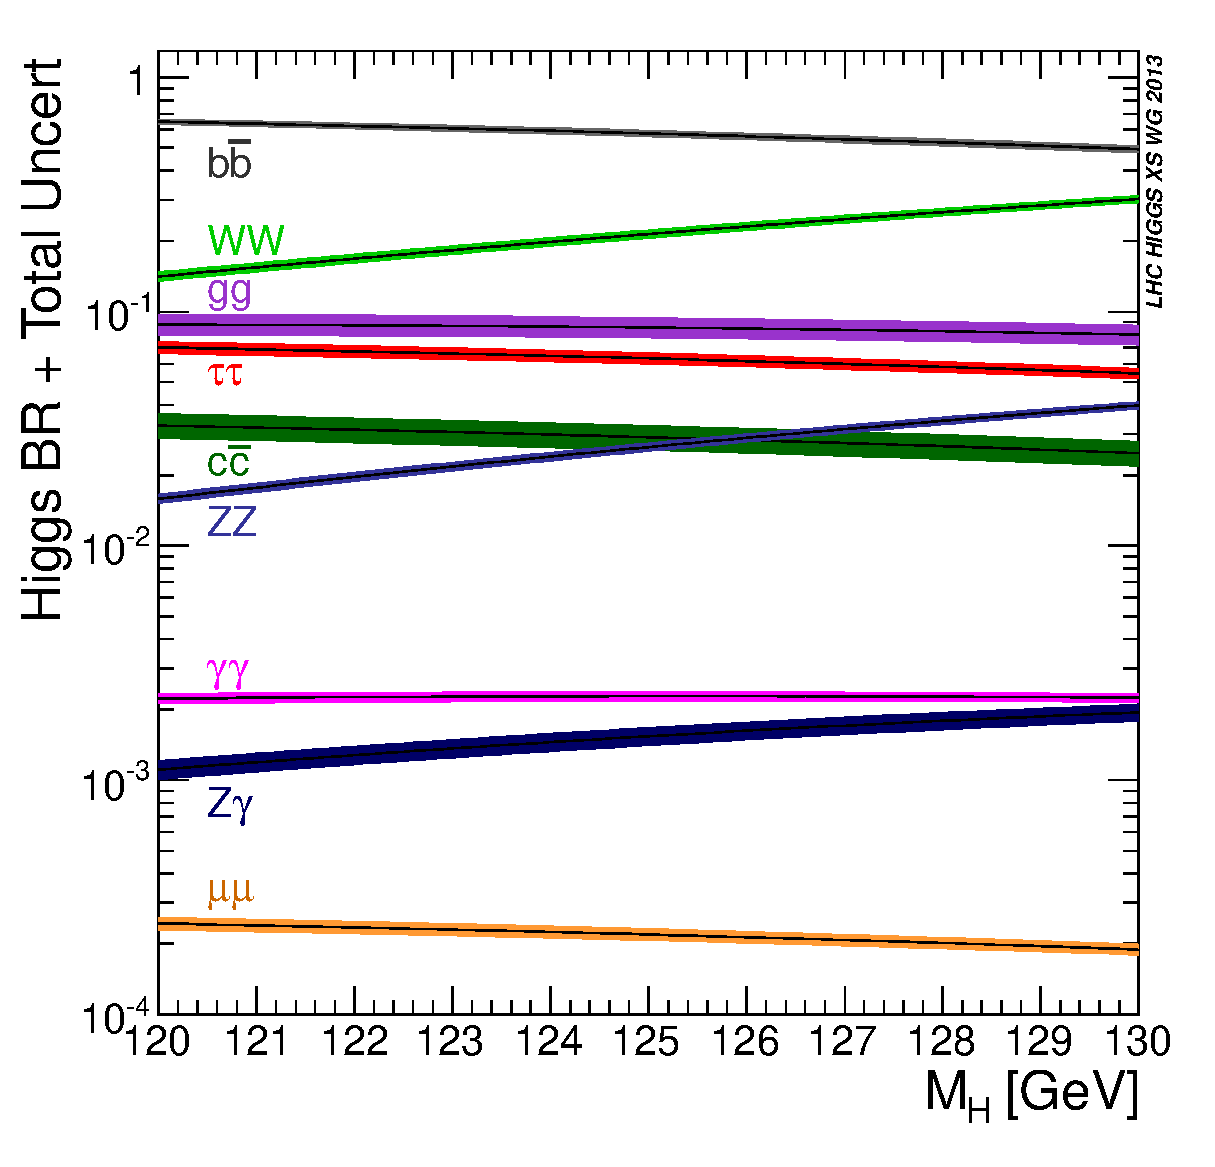
\includegraphics[width=0.4\textwidth]{figures/theory/higgs_br.eps}
\caption[The branching ratios of the Higgs boson]{The branching ratios of the SM Higgs boson around~$m_H = 125$~GeV along with the theoretical uncertainties. Figure from the PDG~\cite{Patrignani:2016xqp}.}
\label{fig:higgs_br}
\end{centering}
\end{figure}

\section{Experimental characterization}
Accurate predictions for the Higgs boson production cross sections and branching ratios for decays allow experimental data to be interpreted and the properties of the Higgs boson to be measured. The mass~$m_H$~has been measured most accurately in the~$\mathrm{H}\rightarrow\mathrm{\gamma}\mathrm{\gamma}$~and~$\mathrm{H} \rightarrow \mathrm{Z}\mathrm{Z} \rightarrow 4\ell$~channels, with a combined value of~$m_H = 125.09 \pm 0.21~(\mathrm{stat}.) \pm 0.11~(\mathrm{syst})$~GeV, dominated by statistical uncertainties, with the photon momentum scale uncertainties being the most significant systematic uncertainty~\cite{Aad:2015zhl}. The spin and parity~$J^P$~of the Higgs boson are probed independently of the mass and total cross section and are found to be compatible with the SM~$0^+$ hypothesis, excluding the pseudoscalar hypothesis at a~$98-99\%$ confidence level~\cite{Khachatryan:2014kca,Aad:2013xqa}. The width of the Higgs boson cannot be measured directly at the LHC, since the mass resolution in the diphoton and~$4\ell$~channels is $1-2$~GeV, 3 orders of magnitude larger than the expected SM line width $\Gamma_H = 4.2$~MeV. However, it can be constrained by comparing the on-shell and off-shell~$\mathrm{H} \rightarrow \mathrm{VV}$~cross sections, thus setting upper limits on~$\gamma_H$~that are around 5-6 times the SM value~\cite{Khachatryan:2014iha}.

It is important to experimentally confirm that the coupling strengths of the Higgs boson to SM particles correspond to those predicted by the SM. Any deviation from the values predicted by the standard Higgs mechanism could thus signal physics beyond the SM (BSM). The simplest way to experimentally characterize discrepancies in the couplings is the so-called~$\kappa$-framework~\cite{Heinemeyer:2013tqa}, where the couplings to SM particles are rescaled by factors~$\kappa_i$~for~$i \in \{\mathrm{Z}, \mathrm{W}, \mathrm{f}, \mathrm{g}, \mathrm{\gamma}, \mathrm{Z\gamma}\}$~which can be determined from signal strength~($\mu = \sigma / \sigma_{\mathrm{SM}}$)~measurements, without modifying the SM structure of the theory. In this formalism, the~\ttH~ signal strength modified is given by~$\mu_{\ttH} = \kappa_{\mathrm{t}}^2$. The CMS and ATLAS collaborations have extracted these signal modifier values from Run I data in a combined fit, with the results shown on~\cref{fig:higgs_kappa}. The results, while compatible with the SM, have significant uncertainties, in particular for~$\kappa_t$, thus paving the way for Run II measurements with improved sensitivity.

\begin{figure}
\begin{centering}
\includegraphics[width=0.8\textwidth]{figures/theory/CMS-HIG-15-002_Figure_015.pdf}
\caption[The Higgs signal strength modifier factors as measured by CMS and ATLAS]{The combined signal strength modified factors~$\kappa$~from the CMS and ATLAS collaborations with Run I data. Figure from~\cite{Khachatryan:2016vau}.}
\label{fig:higgs_kappa}
\end{centering}
\end{figure}

While the~$\kappa$-framework is relatively simple to apply for small deviations in signal strength, the clear short-coming of this approach is that any BSM physics would necessarily change the structure of the theory, rendering the results potentially invalid. In particular, the above approach assumes that the loop contributions in ggF and $\mathrm{H} \rightarrow \mathrm{\gamma} \mathrm{\gamma}$ are not modified by new physics. Furthermore, differences in kinematic distributions, such as the Higgs transverse momentum distribution, cannot be captured in the~$\kappa$~framework. Therefore, it has been suggested to use either Higgs pseudo-observables~\cite{Gonzalez-Alonso:2014eva} or effective field theories (EFT) to further parametrize any deviations from the SM.

\section{Top-Higgs coupling}
In the SM, the coupling between the top quark and Higgs boson is predicted to be~$y_t = \sqrt{2} m_t / v$, which can be verified independently through the measurement of Higgs boson production cross sections. This makes that the direct determination of the top-Higgs coupling in~\ttH~a test of the EWSB model at natural scale where~$y \simeq 1$.  

The top-Higgs coupling plays an important role in vacuum stability, since it controls the evolution of the self-coupling~$\lambda$~of the Higgs potential through renormalization evolution $\frac{\mathrm{d}\lambda}{\mathrm{d}\ln{\mu}}$, where it gives a quartic negative contribution. In particular, if~$y_t$~is sufficiently large but well within the bounds set by experimental uncertainties, the self-coupling~$\lambda$~becomes negative at a renormalization scale~$\mu$~below the Planck scale~$M_{\mathrm{Pl}} = \sqrt{\bar{h}c / G} \simeq 10^{19}~\mathrm{GeV}$, where gravitation becomes important in QFT. This means that the Higgs potential develops an additional minimum, which would possibly make the SM vacuum state metastable, depending on the exact values of~$m_H$~and~$m_t$~\cite{Degrassi:2012ry}. Since the scale where the scalar self coupling becomes negative depends strongly on~$y_t$, an accurate determination of~$y_t$~can help to pinpoint the scale of new physics in the absence of clear BSM signals~\cite{Bezrukov:2014ina}.

Furthermore, the top-Higgs coupling, which is purely scalar in the SM, can be extended quite generally to contain scalar and pseudoscalar interactions, making it possible to use results from~\ttH~for setting direct constraints on anomalous top-Higgs couplings~\cite{Kobakhidze:2016mfx}. Such anomalous couplings can arise from the two-Higgs doublet model that appears in several BSM scenarios, such as supersymmetry or axions~\cite{Branco:2011iw} or from models with a composite Higgs~\cite{Liu:2017dsz}.